\begin{document}

\title {\ZHH \huge TCP的状态}
\author {\small gaccob}
\date {\small 2012 年 8 月 14 日}
\maketitle

\section {\ZHH TCP的流转状态图} {
    {一图胜万言, 先看一下来自UPN的一张图: }\par
    \begin{figure}[htbp]
        \centering
        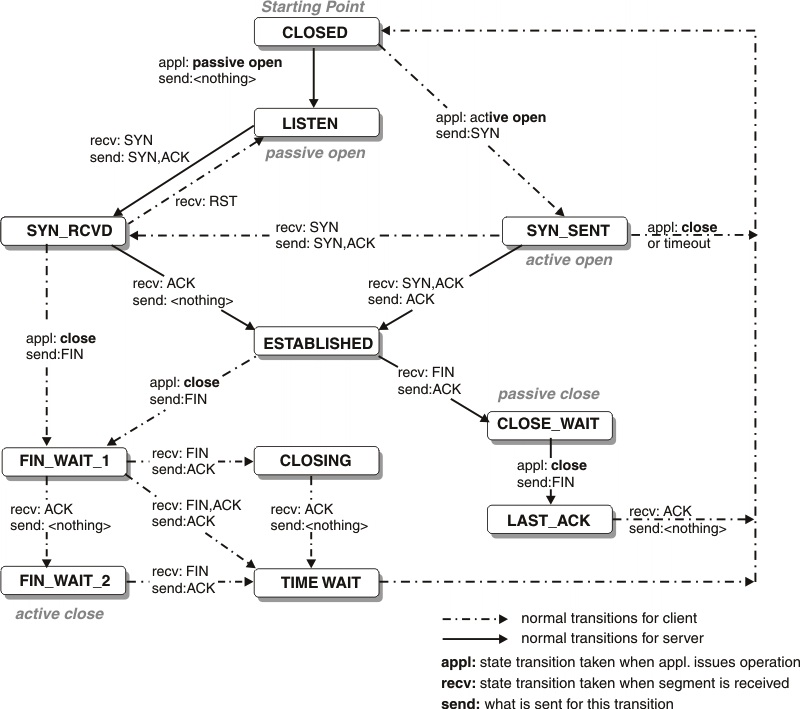
\includegraphics [width=400pt, keepaspectratio] {tcp_status.jpg}
    \end{figure}

    \begin{itemize}
    \item {CLOSED: 无连接状态.}
    \item {LISTEN: server监听端口, 等待连接, 这个叫\textcolor{blue}{passive\_open}.}
    \item {SYN\_RCVD: server收到SYN, 发出SYN, ACK, 等待client ACK.}
    \item {SYN\_SENT: client发出SYN, 请求建立连接, 等待server ACK, 这个叫\textcolor{blue}{active\_open}.}
    \item {ESTABLISHED: 连接建立. }
    \item {FIN\_WAIT\_1: 主动方发送FIN, 主动关闭, 等待server ACK, 这个叫active\_close. }
    \item {FIN\_WAIT\_2: 主动方收到了对方ACK, 继续等待对方FIN.}
    \item {CLOSING: 主动方在\textcolor{blue}{active\_close}的同时, 收到对端的FIN, 这表明了双方同时请求关闭, 这时主动方发出ACK, 继续等待对方ACK. 一般比较罕见. }
    \item {TIME\_WAIT: 主动方收到被动方的FIN并发出ACK之后的状态, 一般会有2MSL, 是为了保证最后一个ACK包不丢失.}
    \item {CLOSE\_WAIT: 被动方收到FIN发出ACK之后就进入这个状态, 等待数据传输完, 到发出FIN之前, 都处于这个状态. 这个叫\textcolor{blue}{passive\_close}. }
    \item {LAST\_ACK: 被动方在CLOSE\_WAIT状态中发出FIN, 则进入LAST\_ACK, 等待对端最后一次ACK确认.}
    \end{itemize}\par

    {需要注意的一点是: 图中的关闭连接的状态流转, 不限定于client或者server, 而是解释为主动方(发起active\_close)或被动方(passive\_close). }\par
    {server从监听->建立连接->被动关闭的典型状态流转: CLOSED->LISTEN->SYNC\_RCVD->ESTABLISHED->CLOSE\_WAIT->LAST\_ACK->CLOSED. }\par
    {client从建立连接->主动断开的典型状态流转: CLOSED->SYN\_SENT->ESTABLISHD->FIN\_WAIT1->FIN\_WAIT2->TIME\_WAIT->CLOSED. }\par
}

\section {\ZHH FIN\_WAIT\_2和CLOSE\_WAIT} {
    {当FIN\_WAIT\_2时, 如果因为对端的程序bug, 或者对端的网络出现故障, 会导致主动方的状态超时, 这时候会直接进入CLOSED状态, 超时时间与tcp\_fin\_timeout参数有关. 特别是当网络中有大量的FIN\_WAIT\_2或者CLOSE\_WAIT时 (一个在主动方, 一个在被动方, 两者是相互对应的), 要注意检查为何收不到FIN, 是不是程序存在bug (一般不太可能是攻击, 因为已经建立了连接, 对攻击者消耗也很大).}\par
}

\section {\ZHH TIME\_WAIT和2MSL} {
    {一般我们会发现主动关闭方有很多TIME\_WAIT的状态, 这是正常的. TIME\_WAIT的超时时间长达2个报文的存活周期, 这有两个原因: 1. 保证最后一个ACK传输到对端(没有重传请求); 2. 保证网络中不会有残留的报文, 被新连接接收而产生数据错乱. }\par
    {对于主动关闭的短连接服务器来说, 可能产生大量的TIME\_WAIT状态, 带来一定程度上资源浪费, 一种方法是设置socket的SO\_LINGER标志位来使socket调用close()之后发送RST来强制终止TCP连接, 但是并不推荐. }\par
    {如果有root权限的话, 推荐的做法是调整内核参数: tcp\_tw\_reuse=1, tcp\_tw\_recycle=1. tcp\_tw\_reuse开启重用, 允许TIME\_WAIT的socket重新用于tcp连接 (只要五元素不一样就不会有问题, 但是如果这时候对端以相同的端口请求建立连接, 则会收到FIN); tcp\_tw\_recycle打开了TIME\_WAIT的socket的快速回收开关, 目测回收时间在1s左右, 一般来说, 单开启tcp\_tw\_recycle已经基本OK了. } \par
}

\section {\ZHH SYN\_RCVD与syn-flood} {
    {当server中出现大量的SYN\_RCVD状态时, 代表了tcp负载过大来不及处理新的连接, 也许是syn-flood攻击(是指攻击方估计发送syn包而不发送ack, 导致tcp连接建立不起来, 从而使服务器长时间停留在SYN\_RCVD状态而消耗服务器资源). 一般碰到这种情况, 可以从/var/log/messages中看到日志, 如果是负载跟不上需要做扩容或者调整负载均衡策略, 如果是异常的攻击行为, 可以通过调整内核参数或者防火墙的黑名单策略来缓解. } \par
    {内核参数tcp\_max\_syn\_backlog: 代表处于SYN\_RCVD状态的socket在队列中的最大数量, 一般默认是1024, 调高这个值可以有效的缓解(注意, 不是解决)小规模的syn-flood. 在负载繁忙的服务器上, 也应该调高这个参数. }\par
    {现代的unix系统中, 普遍采用多队列处理方式, 即一个基本队列维护已经ESTABLISH的socket, 其他半打开的连接, 例如SYN\_RCVD的socket, 在另一个队列. 这样可以很大程度上缓冲syn-flood这种攻击. }\par
    {内核参数tcp\_syncookies: 只有在内核编译时选择了CONFIG\_SYNCOOKIES时才会发生作用, 当出现syn等候队列出现溢出时象对方发送syncookies, 目的是为了防止syn-flood攻击. 这个选项严重违背了tcp协议, 而且会对某些服务导致严重的性能影响(例如smtp转发), 一般不推荐打开. }\par
}

\section {\ZHH BSD socket API与tcp状态} {
    {listen(): 进入LISTEN;}\par
    {accept(): 从已经ESTABLISHED的队列中取出一个来, 队列的大小取决于listen()的参数; }\par
    {close(): 开始进入FIN\_WAIT\_2状态, 等待到TIME\_WAIT; }\par
}

\end{document}
